\documentclass[letterpaper]{article}
\usepackage{underscore}
\usepackage[left=2.0cm, right=2.0cm, top=2.0cm]{geometry}
\usepackage[utf8]{inputenc}
\usepackage{graphicx}
\usepackage{graphics}
\usepackage[spanish]{babel}
\usepackage{lipsum}
\usepackage{float}
\usepackage{subfigure}
\usepackage{biblatex}
\usepackage{csquotes}
\usepackage{color}

\title{Ev\_3\_4\_Diseño y fabricación de 3 PCBs con optoacopladores, transistores y relevadores como dispositivo de interfaz y probarla en la practica 10}
\author{Alcantar Días Joel Alejandro \\\\\\ Carrasco Quiñones Karla Daniela \\\\\\ Ledesma Hernández Miguel Ángel \\\\\\ Reyna Gurrola Marcela}
\date{5/11/2019}

\begin{document}

\maketitle
\vspace{2cm}
\begin{center}
    
\includegraphics[scale=0.4]{IMG/UPZMGlog.png}\\
    \vspace{2cm}
    \begin{large}
        Sistemas electrónicos de interfaz\\
        4-A, Mecatrónica\\
    \end{large}
\end{center}

\newpage
\section{Modelado en Kicad}
\begin{large}
    Para modelar en kicad se crea un archivo nuevo, éste debe ser un esquemático en donde se cargan los componentes del circuito, para posteriormente simular y ver donde puede haber algún fallo, así como para verificar que todo funciona perfectamente.  \\
    Acto seguido, al de terminar el esquematico se crea un plano de PCB en la parte con un "circuito impreso", esta sección es la sección de pcb; en donde se comienza a modelar la PCB, con base a el esquemático creado previamente y el listado de conexiones generado.\\
    Se crea una sección que será la medida de nuestra baquelita, en esta sección irán los componentes. Se introducen los componentes para posteriormente unir por medio de la herramienta Whire (cable)[tecla='W'], las secciones de cada componente que está unido según el listado. Es recomendable cubrir la mayor parte del cobre en la baquelita para un uso mas eficiente del Cloruro Ferrico, para ello se seleccionará la herramienta de Añadir zona. Esta herramienta lo que permite es seleccionar un área en donde no se encuetra nada para poder dejar cobre en esa parte y que el óxido ferrico corroa más facil y rápido la placa.
\end{large}
\section{Técnica de planchado de PCB}
\begin{large}
    Esta técnica consiste en imprimir con toner sobre una hoja de papel Couche delgada, en la cual se imprime el circuito, este papel es parecido al papel de revista, y se tiene que "literalmete" planchar la hoja en la que se imprimio el circuito sobre una baquelita por la parte del cobre  hasta que el toner se adiera a la baquelita, después se sumerge en agua para causar un choque térmico y con esto que se adiera mejor la impresión del circuito a la placa.
\end{large}
\newpage
\section{PCB realizadas.}
\begin{figure}[hbtp]
    \centering
    \subfigure[PCB del circuito con darlington]{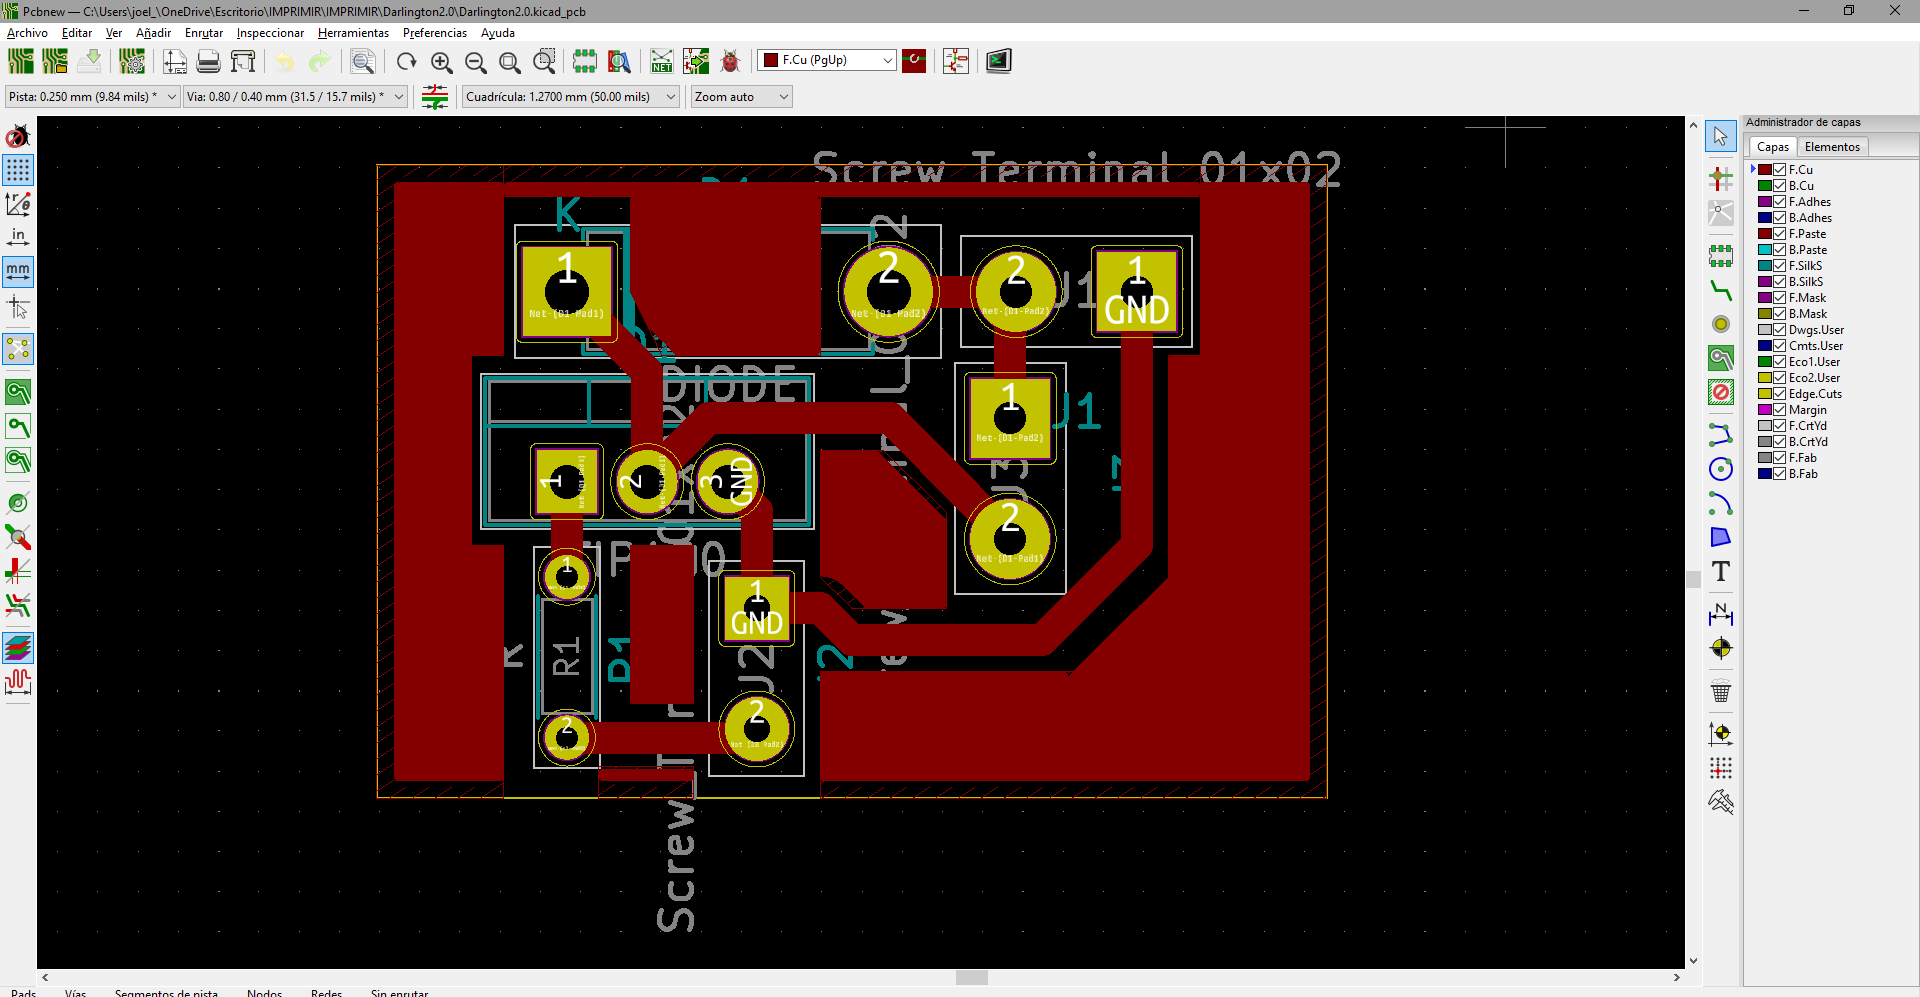
\includegraphics[width=13cm]{IMG/PCB/Darlington.png}}
    \subfigure[Circuito darlington]{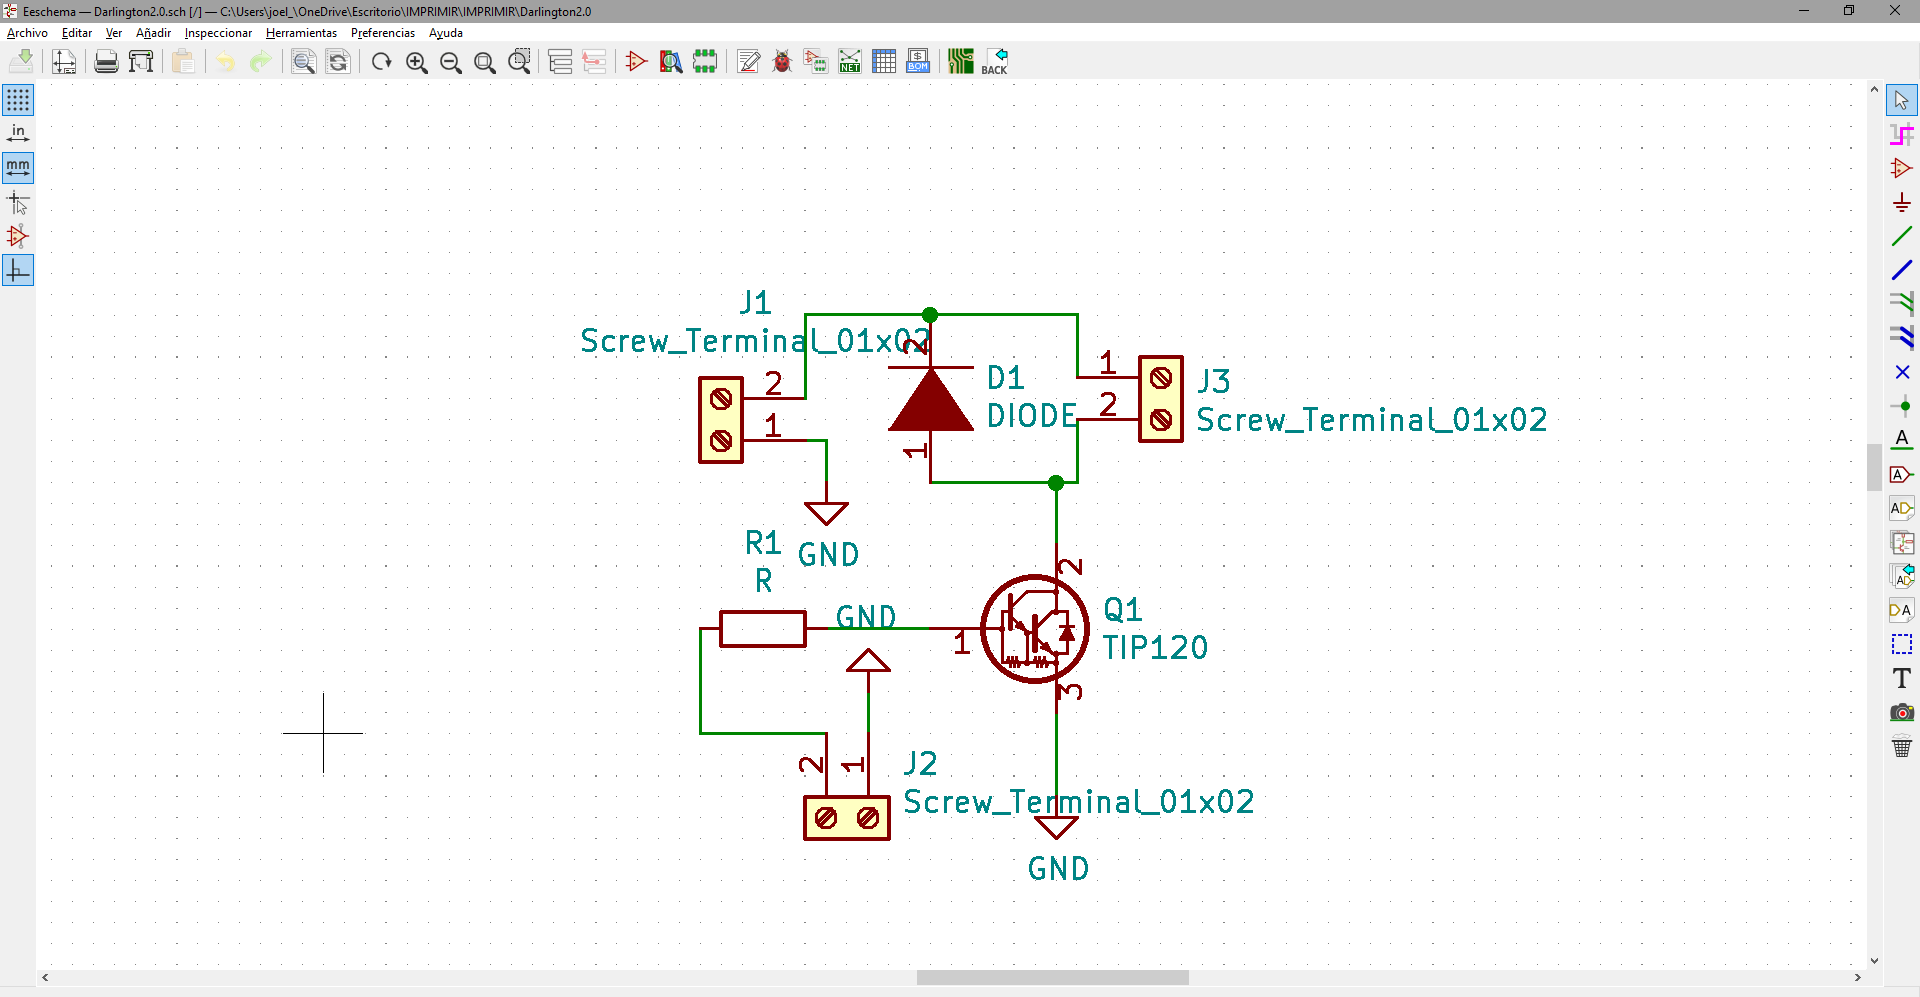
\includegraphics[width=13cm]{IMG/Circuito/Relaysote.png}}
    \caption{Darlington}
    \label{fig:darlington}
\end{figure}

 \begin{figure}[hbtp]
     \centering
     \subfigure[PCB del puente H: ]{\includegraphics[width=13cm]{IMG/PCB/PuenteH.png}}
     \subfigure[Circuito: Puente H] {\includegraphics[width=13cm]{IMG/Circuito/PuenteH.png}}
     \caption{Puente H}
     \label{fig:Puenteh}
 \end{figure}   
 
 \begin{figure}[htbp]
     \centering
     \subfigure[PCB del Circuito sensor de luz]{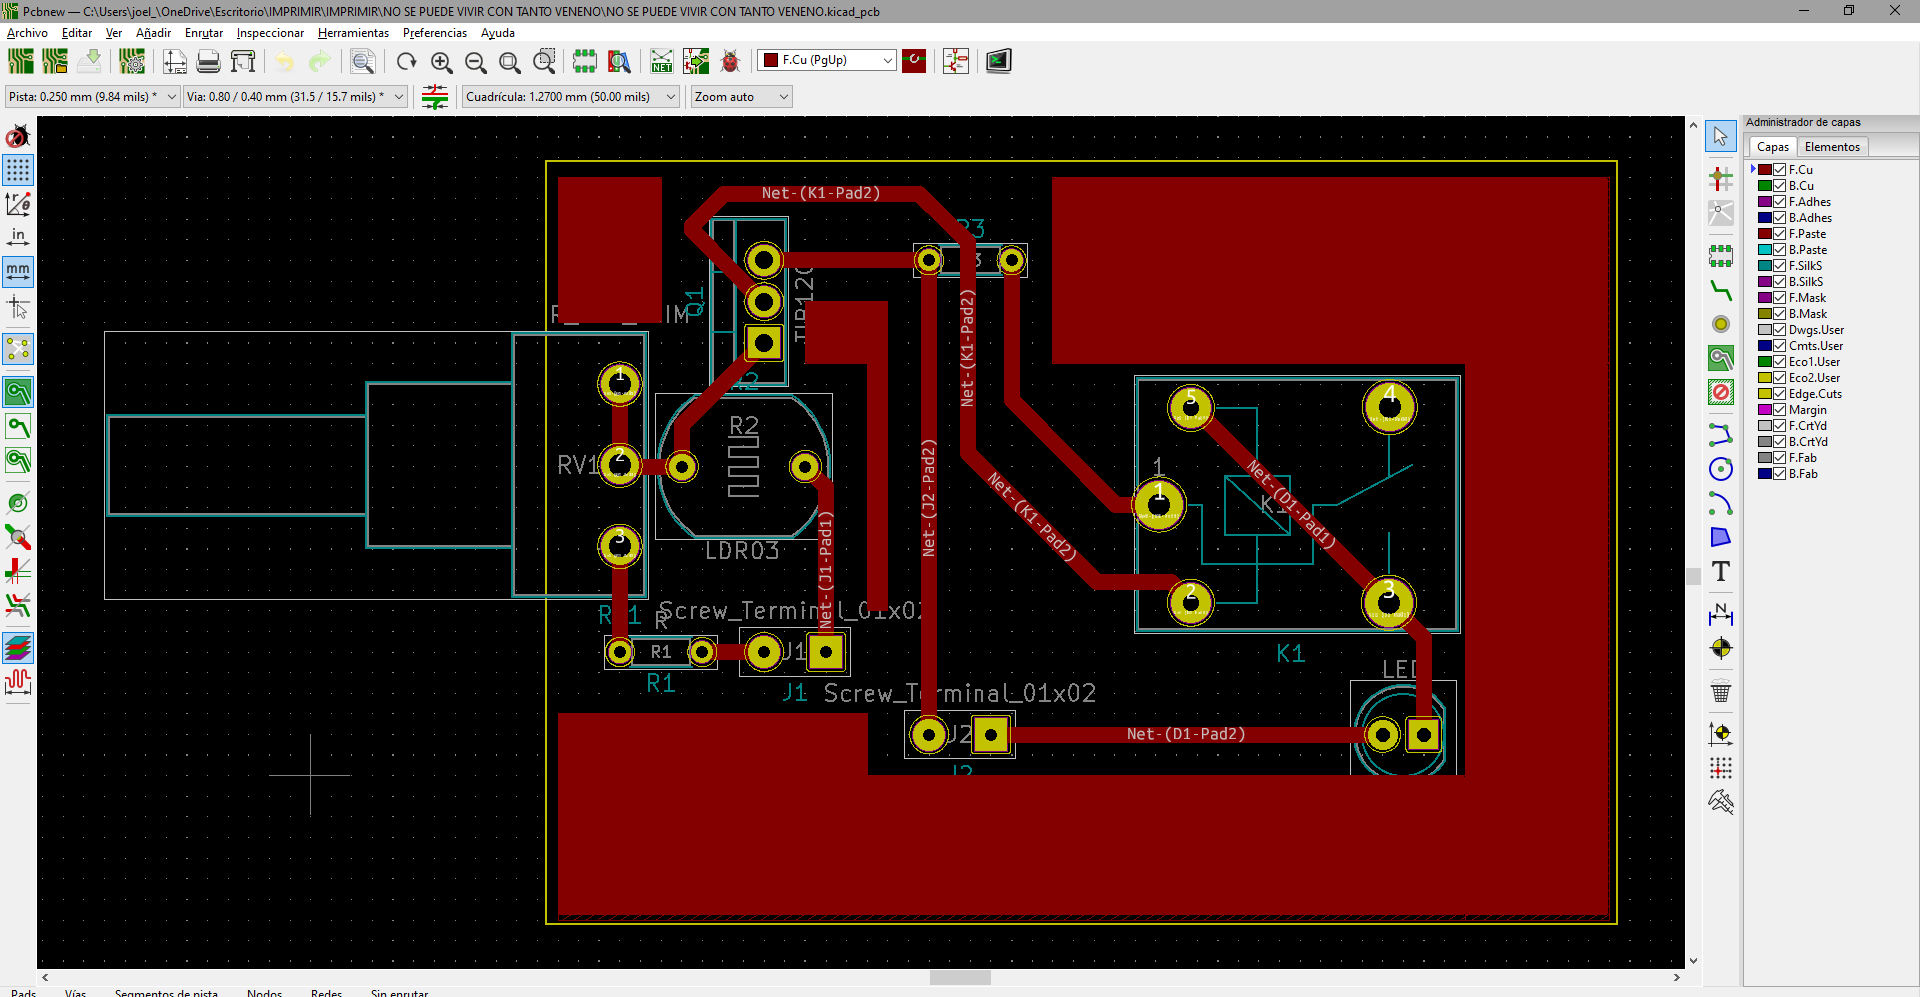
\includegraphics[width=13cm]{IMG/PCB/Sensordeluz.png}}
     \subfigure[Circuito sensor de luz]{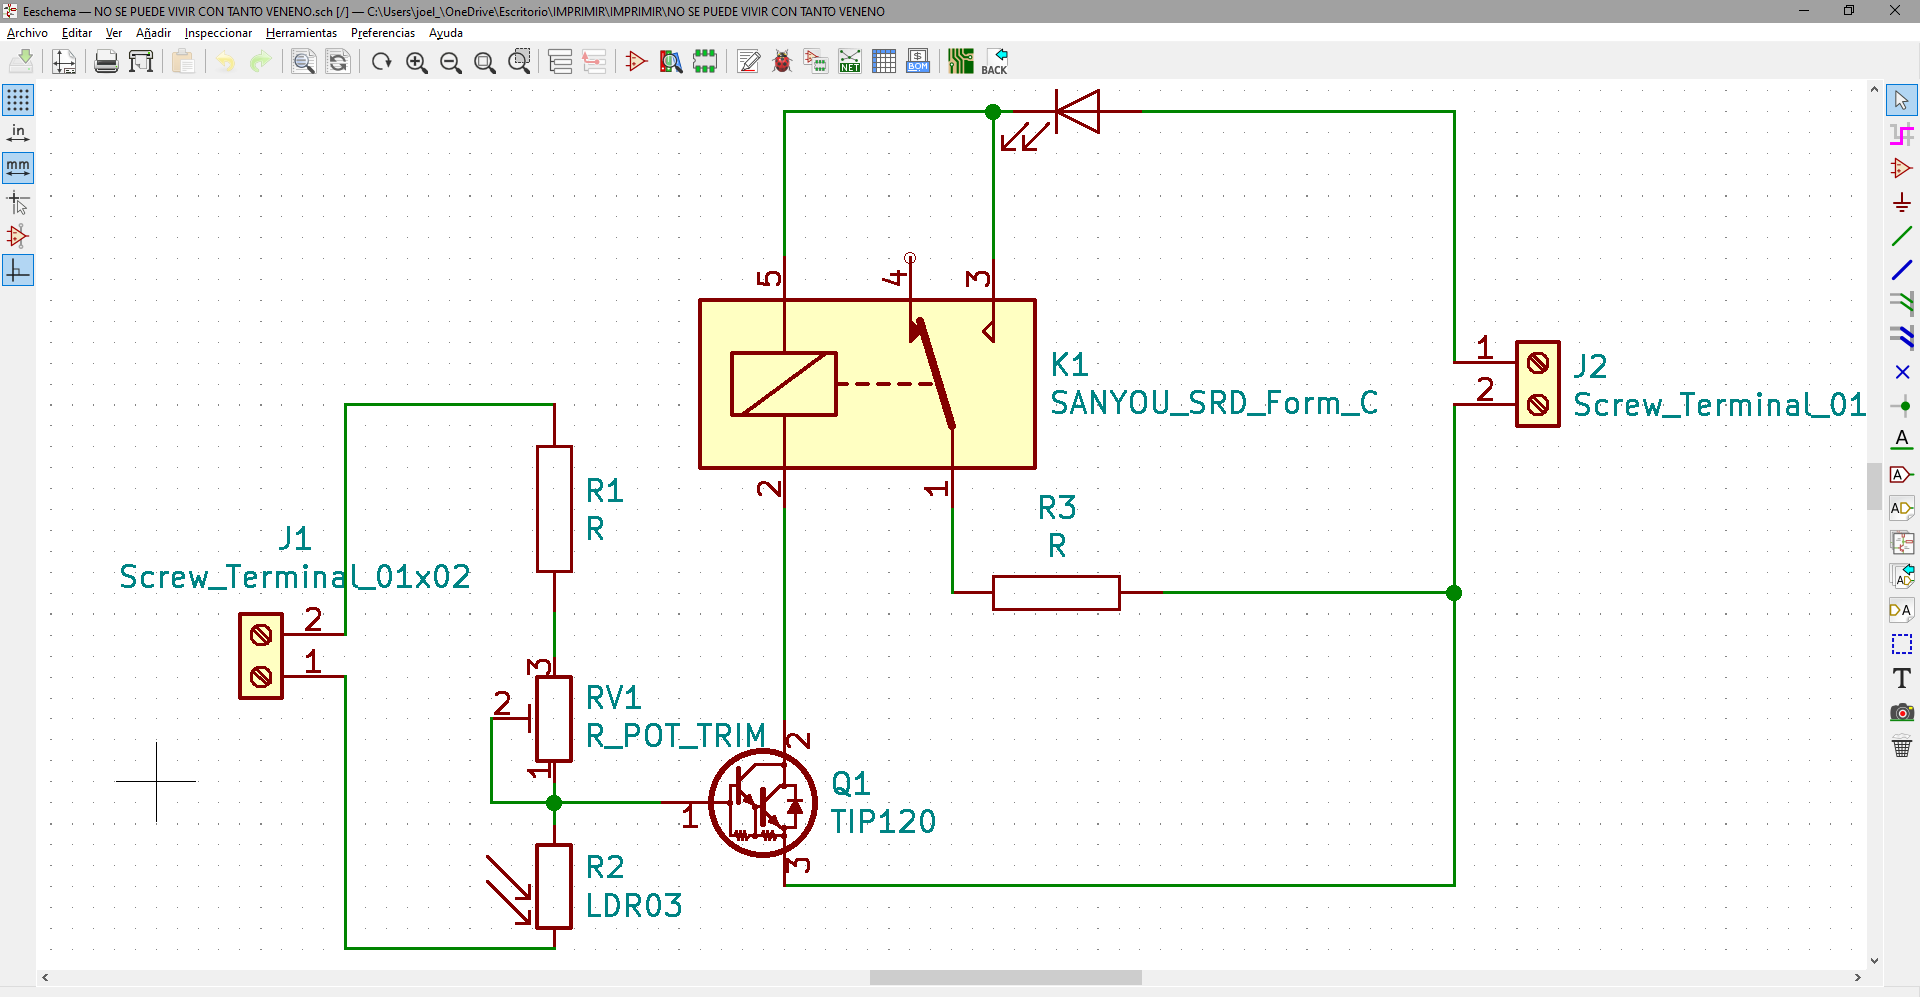
\includegraphics[width=13cm]{IMG/Circuito/Detectordeluz.png}}
     \caption{Sensor de luz}
     \label{fig:LS}
 \end{figure}

\begin{figure}[htbp]
    \centering
    \subfigure[PCB del Módulo relay]{
    \includegraphics[width=13cm]{IMG/PCB/Modulorelay.png}}
    \subfigure[Circuito Módulo relay]{\includegraphics[width=13cm]{IMG/Circuito/Modulorelay.png}}
    \caption{Modulo Relay}
    \label{fig:relei}
\end{figure}

\begin{figure}[htbp]
    \centering
    \subfigure[PCB del Módulo de activación]{
    \includegraphics[width=13cm]{IMG/PCB/Modulodeactivacion.png}}
    \subfigure[Circuito Módulo de activación]{\includegraphics[width=13cm]{IMG/Circuito/Modulodeactivacion.png}}
    \caption{Modulo de activación}
    \label{fig:Activo}
\end{figure}

\begin{figure}[htbp]
    \centering
    \subfigure[PCB del regulador de AC]{
    \includegraphics[width=13cm]{IMG/PCB/Regulaciondefoco.png}}
    \subfigure[Circuito del regulador de AC]{\includegraphics[width=13cm]{IMG/Circuito/Regulaciondefoco.png}}
    \caption{Regulador de AC}
    \label{fig:AClohace}
\end{figure}


\end{document}
